\documentclass{article}
\linespread{1.5}

\usepackage[utf8]{inputenc}
\usepackage[T2A]{fontenc}
\usepackage[russian]{babel}
\usepackage{secdot}
\usepackage{hyperref}
\usepackage{amsmath}
\usepackage{subfig}
\usepackage{subcaption}
\usepackage{float}
\usepackage[top=2cm,right=2cm,bottom=2cm,left=2cm]{geometry}

\title{Учим процессор планировать расход ресурсов}
\author{Альберт Нагапетян\footnote{albert.nagapetyan@phystech.edu} \and Семен Пьянков\footnote{pyankov.sa@phystech.edu}}
\date{}
\bibliographystyle{unsrt}
\addto\captionsrussian{\def\refname{}}

\usepackage{graphicx}
\graphicspath{{/Users/admin/Desktop/}}
\graphicspath{{/}}
\DeclareGraphicsExtensions{.pdf,.png,.jpg}

\begin{document}
\maketitle

\section{Постановка задачи}
В современном мире мы постоянно встречаем и используем  вычислительные устройства, такие как телефоны, компьютеры, мейнфреймы оснащенные процессорами, которые обрабатывают команды, процессы посылаемые операционной системой или гипервизором. В каждый момент времени процессор может делать заданное число операций, что является его скорость. Это число операций делится в некоторой пропорции между доступными для выполнения в текущий такт процессами. Процессор может корректировать скорость своей работы в каждый из $T$ моментов времени. Скорость процессора в каждый момент времени должна лежать в некотором отрезке допустимых значений, а также скорости в два последующих момента времени не могут отличаться по абсолютной величине сильнее чем на некоторое число $R$. Энергия, потребляемая процессором в $i$-ый момент времени, зависит от его скорости $x_i$ в этот момент времени, по закону $\alpha + \beta \mathbb{x_i} + \gamma \mathbb{x_i}^2$. \\

Необходимо минимизировать суммарную энергию, потребляемую процессором, и найти распределение ресурсов по процессам и скоростей по времени.  
Суммарная энергия вычисляется по закону $$W(\mathbf{x}) = \sum\limits_{i=0}^{T-1} \alpha + \beta x_i + \gamma x_i^2,$$ где $x_i$ - скорость процессора в момент времени $i$. Следовательно нужно минимизировать сумму энергий, затраченных за все время работы процессора: $$\min \limits_{\textbf{x} \in X} \sum \limits_{i=0}^{T-1} \alpha + \beta x_i + \gamma x_i^2,$$ где $X$ - допустимое множество.

На скорость $x_i$ накладываются ограничения: $$S_{\min} \le x_i \le S_{\max},$$ где $S_{\min}, S_{\max}$ - заданные минимальная и максимальная скорости. Кроме того, ограничения касаются и приращения скорости, то есть скорости выполнения двух последовательных задач отличаются не более, чем на заданную константу $R$: $$|x_i-x_{i-1}| \le R ~~ \forall i = 1 \dots T-1,$$ где $T$ - суммарное время работы процессора. \\

Скорость в каждый момент времени зависит от того, сколько ресурсов нужно затратить на процессы в каждый момент времени:
$$x_i = \sum \limits_{j=0}^{n-1} X_{ij},$$ где $n$ - общее число процессов, $X_{ij}$ - объем ресурсов, затраченный в $i$-ый момент времени $j$-ым процессом.\\

Кроме того, есть ограничение на суммарную работу, которую должен выполнить процессор: суммарный объём вычислений для каждого процесса должен быть не меньше требуемого для её выполнения\\
$$\sum \limits_{i=0}^{T-1} X_{ij} \ge W_j,$$ где $W_j$ - работа, которую надо затратить для $j$-го процесса, обозначим $\mathbb{W} \in \mathbf{R}^n, \mathbb{W} = \| W_j \|_{j=1}^{n-1}$\\

Получаем задачу:\\
\begin{equation}
\begin{split}
& \min\limits_{\textbf{x}} \alpha T + \mathbf{\pmb{\beta_{*}^{\top}}x} + \gamma \mathbf{x^{\top}x},~ \text{где}~ \ \pmb{\beta_*} \in \mathbf{R^T}, \  \pmb{\beta_*}_i = \beta, \quad  i = 0..T-1 \\
& \text{s.t.} ~\mathbf{x} \succeq \mathbf{S_{min}}\\ 
& \mathbf{x} \preceq \mathbf{S_{max}} \\
& |x_{i} - x_{i-1}| \le R \\
%$\mathbf{x_*} - \mathbf{x^*} \preceq \mathbf{R}$\\
&\mathbf{y} \succeq \mathbf{W},~ \text{где}~ y_j = \sum\limits_{i=0}^{T-1} X_{ij} \\
& x_i = \sum \limits_{j=0}^{n-1} X_{ij} \\
& X_{ij} \geq 0,~ i = 0\dots T-1,~ j = 0\dots n-1\\
\end{split}
\end{equation}


\section{Анализ задачи и описание алгоритмов её решения}

Недостатки постановки - не реализовано в матричной форме. Для краткости записи (да и простоты вычисления) было бы удобнее реализовать в виде матриц и векторов, но не все ограничения позволяют это сделать. Возможно, введя дополнительные переменные, можно было бы реализовать, но между экономией времени работы человека и машины мы решили сделать выбор в свою пользу.\\

Достоинства постановки - составлена задача квадратичного программирования с ограничениями типа равенства и неравенства. Эта задача выпуклая, а значит ее можно решать такими методами как: метод внутренней точки (в нашем случае использовался ECOS $\cite{Domahidi2013ecos}$), ADMM $\cite{Boyd2011}$ (в нашем случае использовался SCS). В общем случае, эти методы решают выпуклые конические задачи, нашу задачу можно свести к задаче SOCP (second order cone problem), это делает cvxpy (функция \text{get\_problem\_data}). Плюсы этих методов в универсальности и отсутствии необходимости подключать какие-либо дополнительные библиотеки, однако некоторые методы не масштабируемы на задачи целочисленного программирования. \\

\section{Результаты экспериментов}

Разные процессы доступны в разные промежутки времени (график допустимости процессов во времени на Рис.~\ref{ris:sched})

\begin{figure}[h]
\center{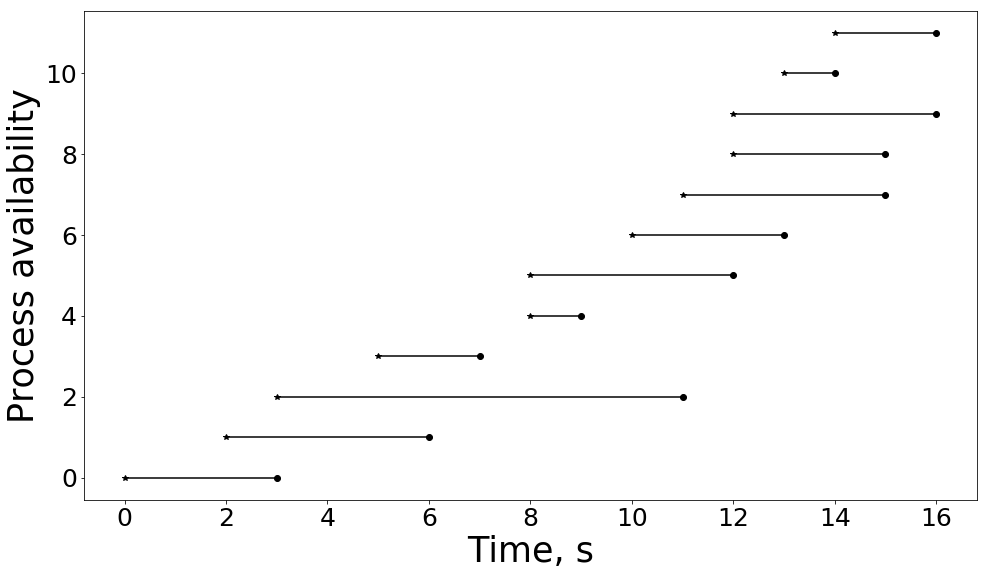
\includegraphics[width=12cm]{sched.png}}
\caption{Зависимость точности от числа итераций}
\label{ris:sched}
\end{figure}

В результате вычислений методами ECOS и SCS мы получили распределение ресурсов по процессам(Рис.~\ref{ris:pow} и Рис.~\ref{ris:speed} ), которое  отличается при решении разными методами, однако оба решения удовлетворяют ограничениям и дают одинаковое суммарное значение энергии. Решения получаются различными, так как они лежат на одной линии уровня, отвечающей минимальному значению функции.\\

\begin{figure}[h]
\subfloat[ECOS]{
    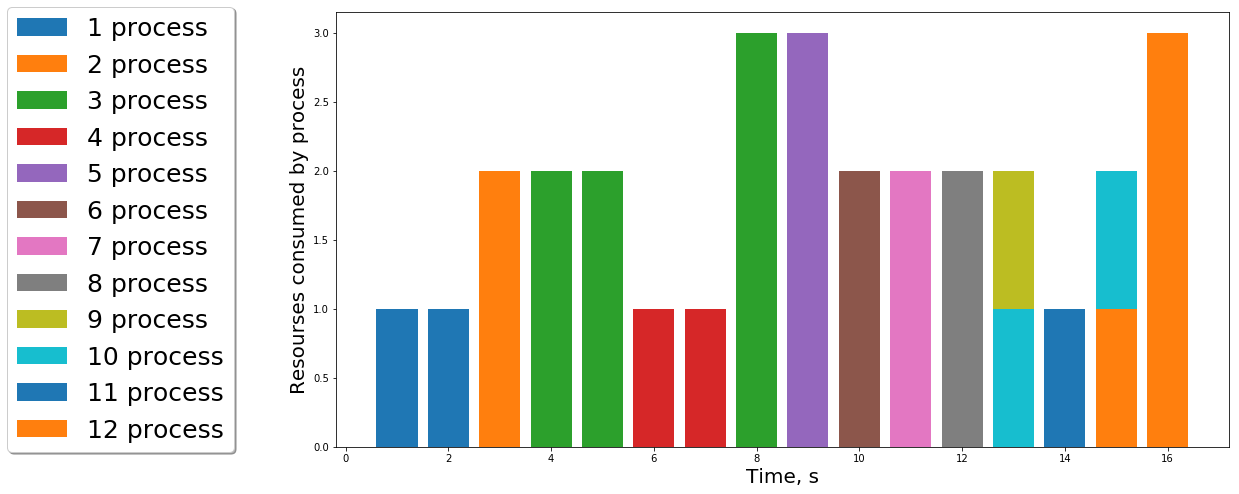
\includegraphics[width=8cm]{ecos_proc.png}
    \label{ris:ECOS_pow}
}
\subfloat[SCS]{
    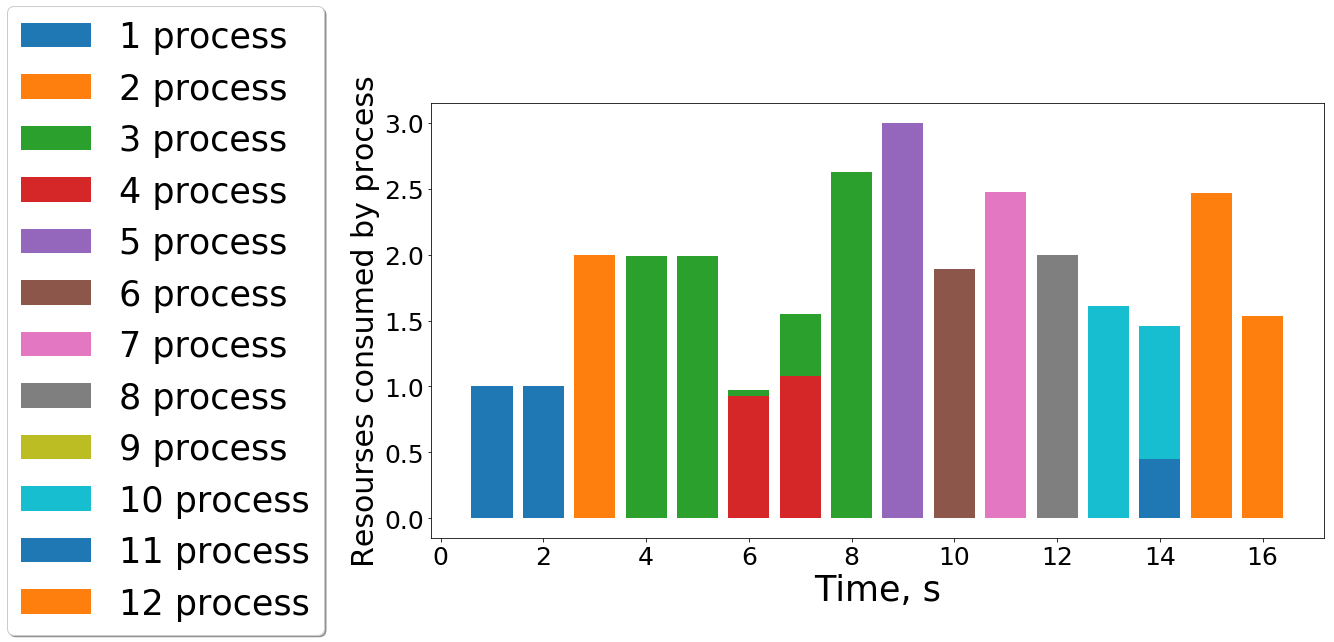
\includegraphics[width=8cm]{scs_proc.png}
    \label{ris:SCS_pow}
}
\caption{Распределение ресурсов по процессам}
\label{ris:pow}
\end{figure}

И значение скорости процессора во времени:\\

\begin{figure}[h]
\subfloat[ECOS]{
    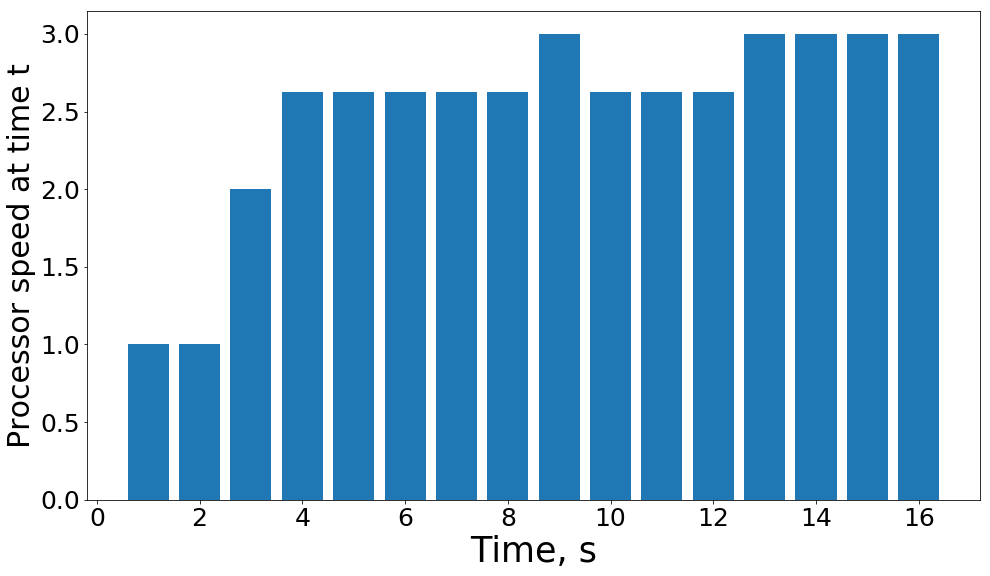
\includegraphics[width=8cm]{ecos_time.png}
    \label{ris:ECOS_speed}
}
\subfloat[SCS]{
    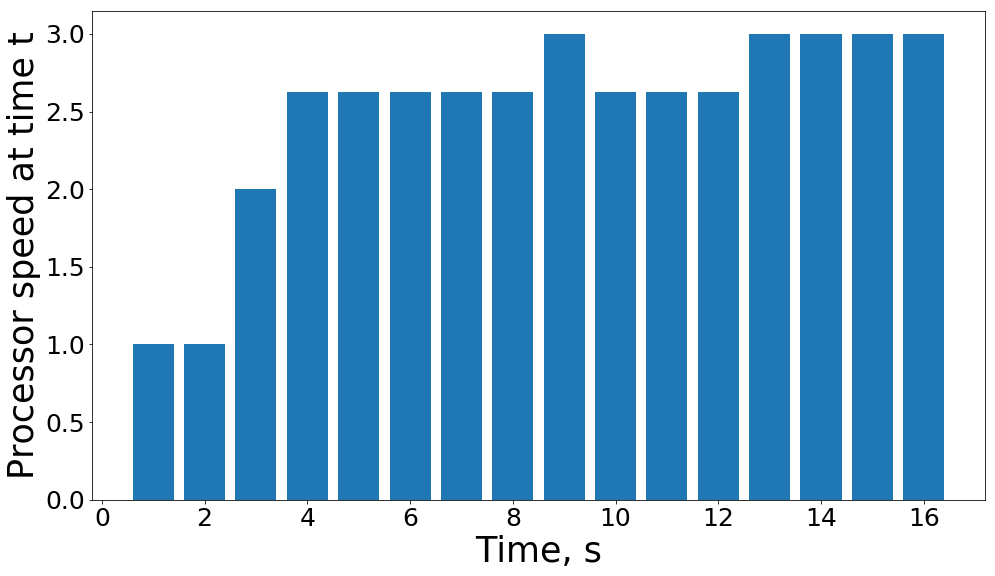
\includegraphics[width=8cm]{scs_time.png}
    \label{ris:SCS_speed}
}
\caption{Распределение скорости процессора}
\label{ris:speed}
\end{figure}


Также была оценена зависимость точности вычисления от числа итераций, см. Рис.~\ref{ris:PREC_iter}

\begin{figure}[h]
\center{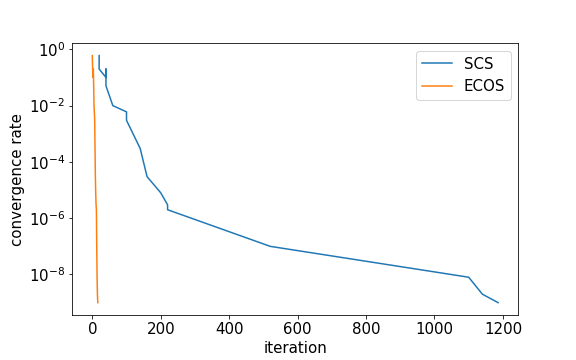
\includegraphics[width=12cm]{cmp_1.png}}
\caption{Зависимость точности от числа итераций}
\label{ris:PREC_iter}
\end{figure}
\\
$~$
\\
$~$
\\
Сравнение SCS и ECOS при решении задачи с точностью $10^{-9}$:

\begin{center}
\begin{tabular}{c|c|c|c}
     &  \# iter & Total time, ms & Dual gap \\
     \hline
     ECOS & 16 &110 & $9\cdot{10^{-7}}$ \\
     \hline
     SCS & 1186 & 129& $2.4\cdot{10^{-12}}$ \\
\end{tabular}
\end{center}

Получили, что ECOS нужно сделать гораздо меньше итераций, чем SCS, для достижения заданной точности (как это видно из графика на Рис.~\ref{ris:PREC_iter}), также скорость выполнения SCS ниже, то есть выгоднее пользоваться ECOS (метод внутренней точки). Также получили оценки зазора двойственности: $9\cdot{10^{-7}}$ для ECOS и $2.4\cdot{10^{-12}}$ для SCS, т.е. при решении методом SCS зазор двойственности меньше. 

Однако, после некоторых раздумий, было принято предположение, что нагрузка (равно как и скорость) процессора должна быть целочисленная. Тогда была найдена модификация ECOS - ECOS\_BB, результат можно видеть на Рис.~\ref{ris:ECOSBB_pow} и Рис.~\ref{ris:ECOSBB_speed}.

\begin{figure}[h]
\subfloat[Распределение нагрузки]{
    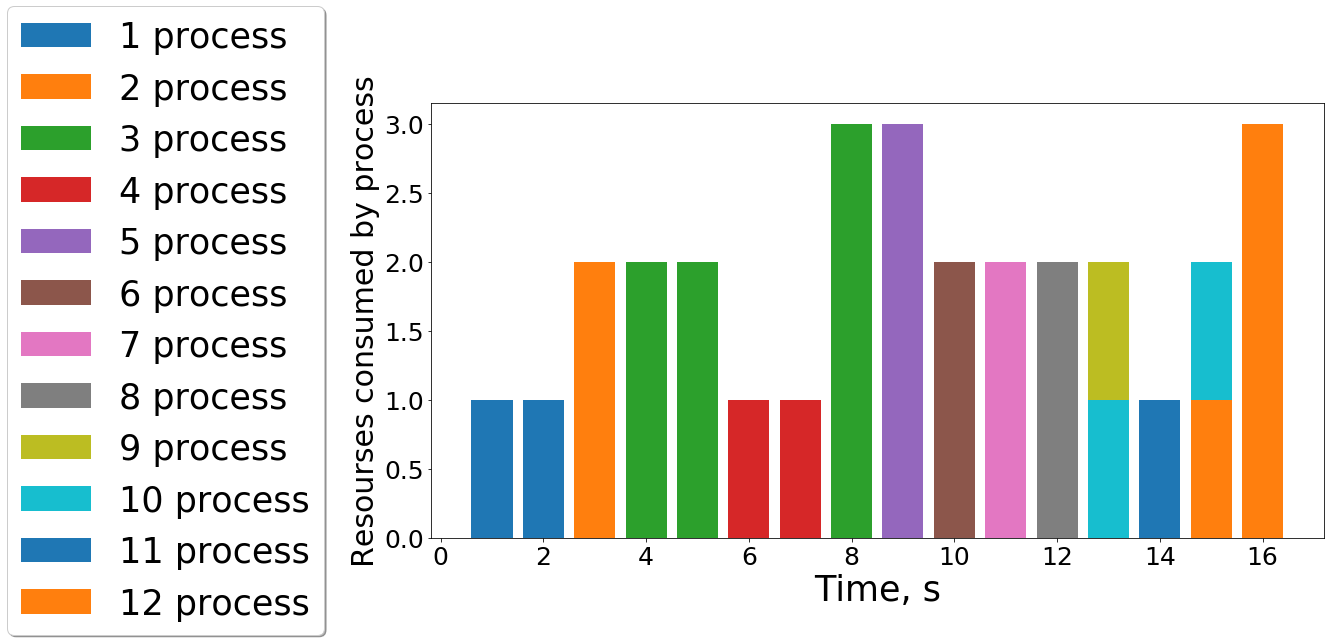
\includegraphics[width=10cm]{ecosbb_proc.png}
    \label{ris:ECOSBB_pow}
}
\subfloat[Скорость]{
    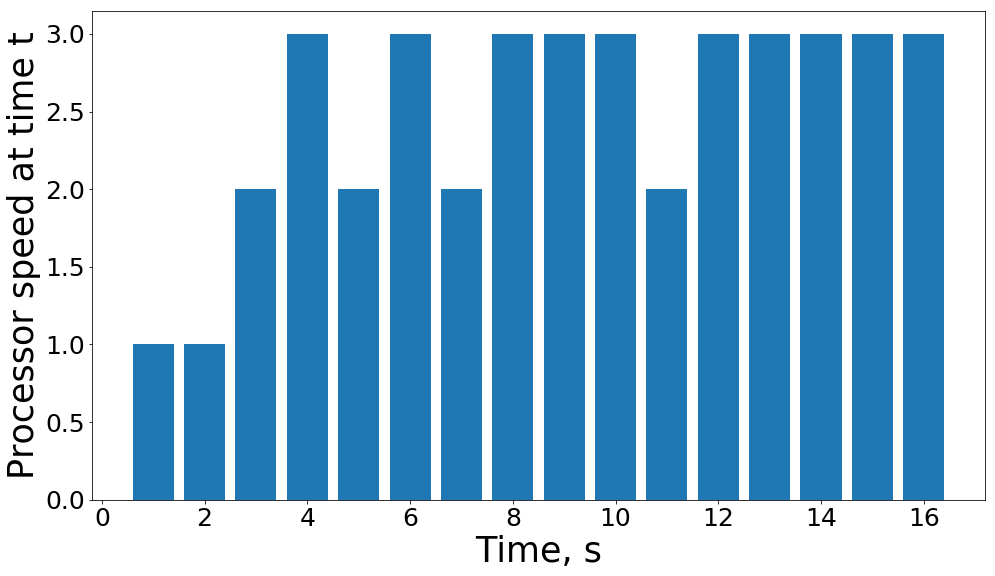
\includegraphics[width=8cm]{ecosbb_time.png}
    \label{ris:ECOSBB_speed}
}
\caption{ECOS\_BB}
\end{figure}

\section{Обсуждение}

В проекте было найдено распределение энергии и скорости процессора в каждый момент времени (в том числе и для целочисленного случая - более приближенного к реальности).

При решении возникла проблема с составлением задачи математического программирования. Чтобы упростить выражение, хотелось получить векторно-матричную форму записи. Но это не будет иметь особого смысла ($\succeq$ реализуется все равно поэлементно, да и не очень понятно, как оформить ограничение $|x_i-x_{i-1}| \le R$ без введения дополнительных переменных). \\

Еще одна трудность - предположение целочисленности задачи. Из-за этого пришлось использовать ECOS\_BB, который, конечно, дал решение, отличающееся от непрерывного случая: отличается как распределение нагрузки (это можно видеть, если сравнить график на Рис.~\ref{ris:ECOSBB_pow} с графиками на Рис.~\ref{ris:ECOS_pow} и Рис.~\ref{ris:SCS_pow}), так и распределение скоростей по времени (видно при сравнении графика на Рис.~\ref{ris:ECOSBB_speed} с графиками на Рис.~\ref{ris:ECOS_speed} и Рис.~\ref{ris:SCS_speed}). Решение, полученное для непрерывной задачи, дает меньшие затраты энергии 162.1 в сравнении с 163.9, полученными при решении целочисленной задачи, но на практике такое распределение вряд ли будет столь экономично. Поэтому для реального применения целочисленное решение выглядит более приемлемым. Скорее всего, при достаточно больших затратах, непрерывный случай будет точнее отображать реальные условия и отличие дискретного решения от непрерывного не будет отличаться так сильно. \\

При первом прочтении условия показалось, что задача достаточно узкая, поскольку нужно знать точное расписание занятости процессора (то есть нужно знать, какие требуется запустить процессы в какое время и на какое время). Но как высяснилось, бывают и такие системы$\cite{Tanenbaum}$. К тому же, если не вдаваться в подробности, то планировщик операционной системы примерно так и составляет расписание (конечно, задача усложняется тем, что мы не знаем, какие к нам придут задачи в будущем, но те задачи, которые известны, распределяются с минимальным потреблением ресурсов). В целом это сильно упрощенная задача, но можно попытаться её обобщить на многопоточную архитектуру, учесть ограничение на число процессов и попробовать реализовать решение задачи для реального планировщика (хотя в действительности проще пользоваться готовыми алгоритмами планирования, например из невытесняющих это FIFO, из вытесняющих - циклическая).\\

Кроме того, в многопоточных системах при использовании пула потоков возникает необходимость в статическом планировании. Потоки для фрагментов задания будут определяться заранее, наше решение поможет оптимизировать это распределение.\\

Еще одно применение - распределение задач в проекте внутри команды. Только необходимо ограничить число одновременно-запущенных процессов числом членов команды (или какой-то величиной, зависящей от этого числа).

\section{Список литературы}
\bibliography{CPUlibNEW}

\section{Роли}

\subsection{Формализация задачи (составление задачи математического программирования)} --- Семен Пьянков, Альберт Нагапетян
\subsection{Реализация на Python:}
    \subsubsection{Поиск алгоритмов, которые позволяют решить эту задачу} --- Альберт Нагапетян, Семен Пьянков
    \subsubsection{Написание кода, решающего задачу с использованием этих алгоритмов} --- Альберт Нагапетян
    \subsubsection{Отладка} --- Альберт Нагапетян %:) как будто мы ей занимаемся 
\subsection{Обоснование решения} --- Семен Пьянков, Альберт Нагапетян
\subsection{Оформление отчета} --- Семен Пьянков
\subsection{Внесение правок в отчет} --- Выполнялось поровну каждым участником
\subsection{Создание корректно оформленного репозитория на Github} --- Семен Пьянков\\

На самом деле разделение очень условное, поскольку вносились изменения разного плана всеми участниками во все части проекта.\\



\end{document}
